\begin{figure} [h]
    \centering
    \includegraphics[scale=0.5]{figures/fig5.png}
    \caption{\textbf{Top:} Signal acquisition circuit. \textbf{\textit{Left:}} Low-noise 5\,V power supply for all SiPM PCB boards (TPS7A470, $4\,\mu\text{V}_\text{RMS}$). \textbf{\textit{Middle:}} 24-channel digital signal reader with FPGA (ICE40HX1K), 5\,V to 3.3\,V level shifters, and indicator LEDs associated with each SiPM sensor. \textbf{\textit{Right:}} Breadboard: Arduino Nano for serial data communication over USB to the computer, and STM32F103C for clock signal generation. \textbf{Bottom left:} Work in progress FPGA detector module. \textbf{Bottom right:} Manual soldering of individual wires for the 24 LED indicators.}
    \label{fig5}
\end{figure}


\begin{figure}[h] 
    \centering 
    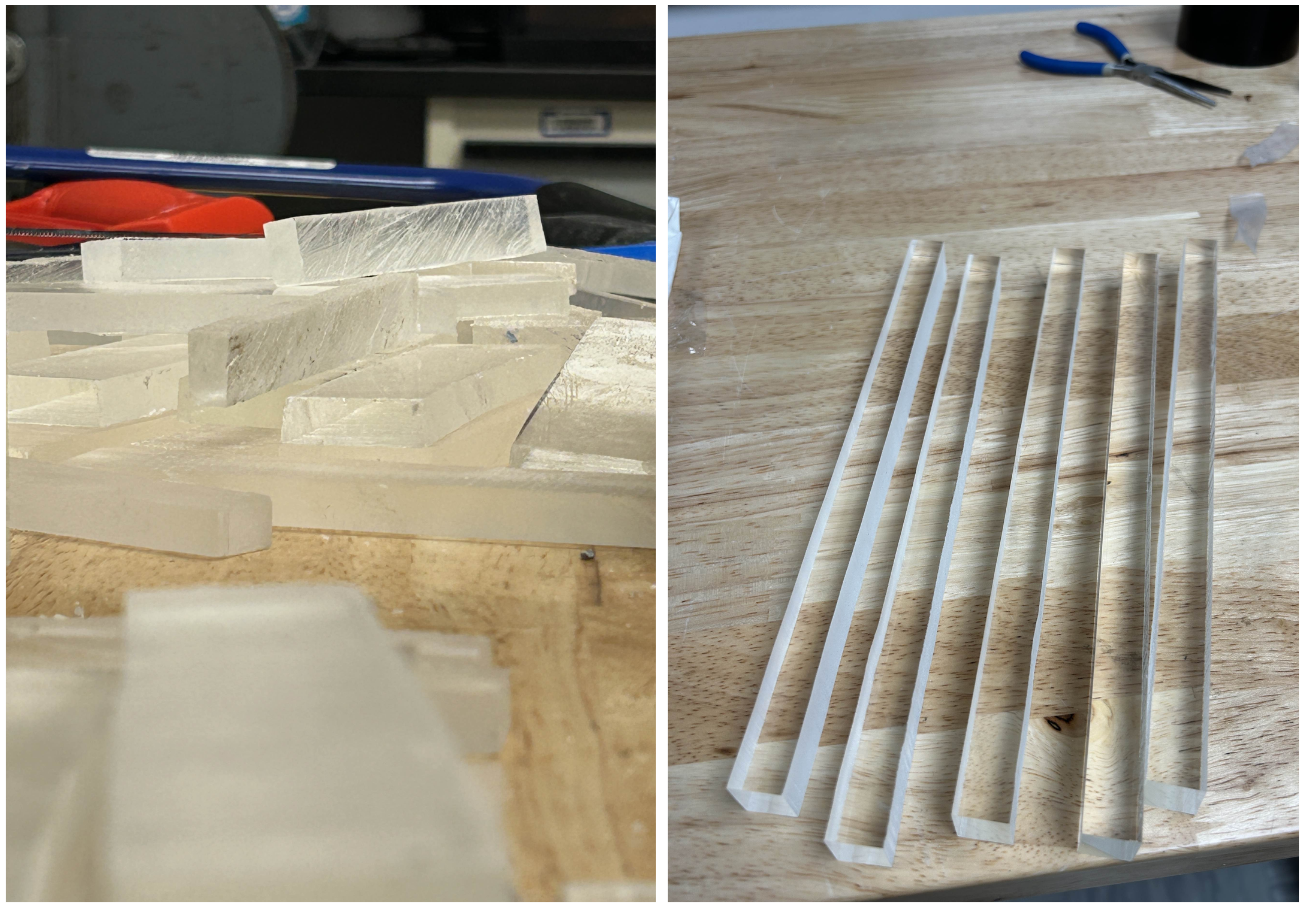
\includegraphics[scale=0.6]{figures/fig6.png}
    \caption{Scintillator rods cut with a bandsaw from a larger
scintillator block. Two $500\times250\times30$ mm BC408 PVT scintillators were graciously offered to us by McGill Professor Dr. David Hanna\textemdash which we then proceeded to cut and polish manually.}
    \label{fig6}
\end{figure}



